\chapter{Flip Flop y Latch}
%\stepcounter{chapter}

%\documentclass{article}
%\usepackage{graphicx}

En este ejercicio se implementaron 2 circuitos, el \textit{gated latch SR} y el \textit{flip flop D}, ambos fueron diseñados sobre una placa multiperforada sobre los cuales se realizaron determinadas mediciones para luego comparar dichos valores con sus versiones disponibles en el mercado.
\section{Gated latch SR}
Existen distintos diseños para el gated latch SR, el que se llevo a cabo fue el diseño visto en la cursada de materia el cual consiste de 2 compuertas AND en conjunción con 2 NOR como se muestra en el siguiente diagrama.
\begin{center}
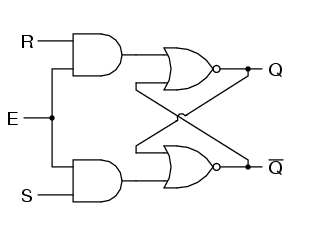
\includegraphics[scale=0.5]{../6-FlipFlop&Latch/E3 ej6 latch SR.png}
\end{center}
Para realizar las funciones de las compuertas lógicas se utilizaron los circuitos integrados 74HC08 y 74HC02 siendo el primero un conjunto de compuertas AND mientras el segundo de NOR, ambos de tecnología CMOS de modo tal de no tener problemas de compatibilidad. Una vez obtenido el circuito se realizaron las mediciones de sus respectivas tensiones de entrada y salida las cuales se muestran en el siguiente cuadro en comparación a su contraparte comercial:
\begin{table}[]
\begin{tabular}{lll}
Gated latch SR            & Diseño propio & Diseño comercial \\
High-level input voltage  & 3.15V         & 2V               \\
Low-level input voltage   & 1.35V         & 0.8V             \\
High-level output voltage & 5.11V         & 3.4V             \\
Low-level output voltage  & -20mV         & 0.2V            
\end{tabular}
\end{table}
\section{Flip-flop D}
Siendo que ya se tenia a disposición el gated latch SR diseñado se decidió crear un pequeño modulo adicional el cual unido al latch pudiese ser operado como un flip-flop tipo D.
Para esto se debió implementar un detector de flancos como es típico en los circuitos de este tipo, como la tecnología utilizada hasta aquí consistía de CMOS se decidió continuar con esta con lo cual se hizo uno de un par de integrados 74HC04 los cuales consisten de conjuntos de compuertas inversoras, o NOT, esto resulto ser un inconveniente ya que la tecnología CMOS al poder realizar operaciones de manera tan acelerada en relación con otras tecnologías no permitía generar un retardo apreciable en la señal clock de entrada. Por esta razón se debieron usar 2 circuitos integrados de este tipo en lugar de únicamente 1, haciendo pasar la señal clock por 11 compuertas NOT hasta tener un flanco apreciable el cual se muestra en la siguiente imagen:
\begin{center}
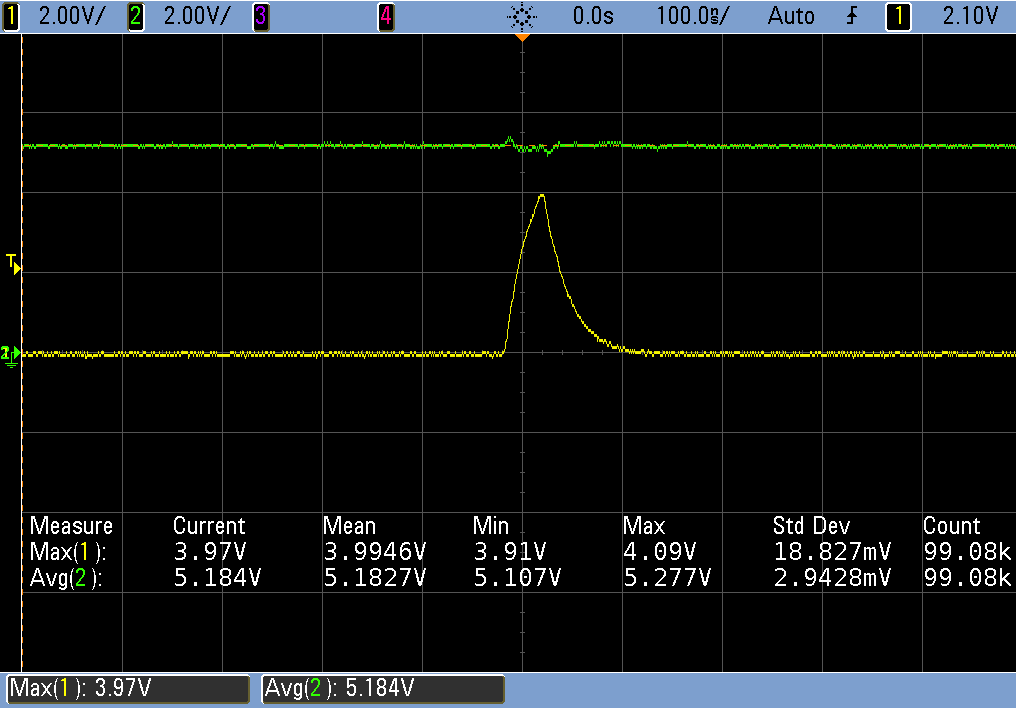
\includegraphics[scale = 0.5]{../6-FlipFlop&Latch/e3_ej6_ed.png}
\end{center}
Dado que el flaco obtenido posea un máximo de tensión de 4V y una duración en promedio de aproximadamente 50ns se debió consultar los datasheets de los integrados utilizados para verificar que pudiesen operar con tal señal. Afortunadamente los integrados utilizados poseen un \textit{High-level input voltage} inferior a los 4V y un \textit{Transition Time} con un valor máximo de 13ns, con lo cual se logró trabajar con dicha señal sin problema.
Por ultimo para la implementación de la compuerta D se utilizó el 74HC00, un circuito integrado de NANDs que ya se había utilizado para el \textit{edge detecter} anterior junto con la compuerta NOT sobrante.
Ahora se muestran las mediciones obtenidas nuevamente haciendo comparación con un flip-flop D comercial:
\begin{center}
\begin{table}[]
	\begin{tabular}{lll}
	Flip-flop D               & Diseño propio & Diseño comercial \\
	High-level input voltage  & 3.15V         & 2V               \\
	Low-level input voltage   & 1.35V         & 0.8V             \\
	High-level output voltage & 5.18V         & 3.4V             \\
	Low-level output voltage  & -23mV         & 0.2V            
	\end{tabular}
\end{table}
\end{center}
\section{Conclusiones}
Como se puedes observar los resultados de las mediciones resultaron bastante distintas a los valores que se esperaría en cuanto a la versión comercial, esto sin embargo es entendible ya que como ya se menciono la tecnología de compuertas implementadas es de tipo CMOS el cual tiene prestaciones distintas a la tecnología utilizada por el \textit{gated latch SR} y el \textit{Flip-flop D} comerciales encontrados, los cuales hacen uso de otro tipo de transistores.